\subsection{Cosmogenic Activation of the Stainless Steel}
\label{secCosmogenicActivationSteel}

Cosmogenic activation of the 316Ti stainless steel used by the XENON100 experiment, in particular, contamination of $^{54}$Mn, has been identified with radioactive screening (see Section~\ref{secScreening}). However, measured samples, even though they are from the same batch, do not provide the full activation history. The material which has been used for the detector construction (see Section~\ref{secDetectorDesign}) has been exposed to cosmic rays for a longer time, due to machining, storage and assembly of the detector components above ground. In addition, some of the parts, such as support rings for the electrode meshes, have been transported a few times by air, thus have been exposed to cosmic rays with a higher flux.

A comprehensive study of the cosmogenic activation in 316Ti SS has been performed within the GERDA double-beta search experiment, which purchased the material from the same provider as XENON100. The study has been published in Ref.~\cite{SteelCosmogenics}, and the main production channels for cosmogenic radionuclides in the stainless steel from Ref.~\cite{SteelCosmogenics} are shown in Table~\ref{tabSteelCosmogenics1}. The measured  production rates (saturation activity) of cosmogenic radionuclides of exposed samples are presented in Table~\ref{tabSteelCosmogenics2}. The activation of the steel samples has been performed at LNGS altitude, 985~m above sea level (latitude 42.25$^{\circ}$N), and the radioactive contamination has been measured with Ge $\gamma$-ray spectrometers installed in the underground laboratory~\cite{SteelGerda}. The production rates at sea level have been calculated by normalization to the lower neutron flux compared to LNGS surface, with a factor 2.4~\cite{PRnormalization}.

%Using only the sources described in the previous sections, the background model shows a deficit in the 700-1100 keV range. Most of this deficit can be explained by cosmogenic activation of the stainless steel parts during materials storage and the detector construction at the ground level, in particular, 54Mn isotope with the half-life time of 312 days. The activity assumed in the present study is 1.25 mBq/kg, and the decays have been generated uni- formly in all parts made of 316Ti SS. This value is well below the conservative limit (2.14 mBq/kg), assuming the production rate of 54Mn in 316Ti SS at LNGS altitude of 6:5 ` 0:7 mBq=kg [17], and taking into account that in Fall 2009 the detector had been underground almost 500 days. Radioactive	isotopes	58 Co,	56 Co,	and	46 Sc	can	be	also produced by cosmic rays in the stainless steel and emit high energy  rays. Their decays have been included in the background model assuming saturation activities at LNGS altitude [17]. However, due to short half-life times of $80 days their contribution is negligible. The predicted background from the cosmogenic activation in the stainless steel	is	at the	level	of	10?4 events  kg?1  day?1  keV?1, thus about 5\% of that from natural radioactivity in the same components.

\begin{table}[!h]
\centering
\caption[Cosmogenic production of radioactive isotopes in 316Ti stainless steel]{Cosmogenic production of radioactive isotopes in 316Ti stainless steel~\cite{SteelCosmogenics}.}
\label{tabSteelCosmogenics1}
%\vspace{0.2cm}
\begin{tabular}{>{\footnotesize}l|>{\footnotesize}l|>{\footnotesize}c}
%\begin{tabular}{l | l | c }
\hline
Isotope				& Production channel													& T$_{1/2}$ [days]	 \\
\hline
$^{54}$Mn			& $^{56}$Fe(n,p2n), $^{56}$Fe($\mu^{-}$,$\nu$2n)								& 312.23 \\
$^{58}$Co 			& $^{60}$Ni(n,p2n), $^{60}$Ni($\mu^{-}$,$\nu$2n), $^{58}$Ni(n,p) 					& 70.83 \\
$^{56}$Co 			& $^{58}$Ni(n,p2n), $^{58}$Ni($\mu^{-}$,$\nu$2n) 								& 77.236 \\
$^{46}$Sc 			& $^{48}$Ti(n,p2n), $^{48}$Ti($\mu^{-}$,$\nu$2n), spallation on Fe 					& 83.788 \\
$^{48}$V 				& $^{52}$Cr(n,p4n), $^{50}$Cr(n,p2n), $^{50}$Cr($\mu^{-}$,$\nu$2n), spallation on Fe 	& 15.9735 \\
\hline
\end{tabular}
\end{table}


\begin{table}[!h]
\centering
\caption[Cosmogenic production in the 316Ti stainless steel from the measurements and Monte Carlo simulations]{Cosmogenic production in the 316Ti SS from the measurements~\cite{SteelCosmogenics} and Monte Carlo simulations. The production rates at LNGS level have been measured, and inferred for sea level from these measurements using a factor 2.4~\cite{PRnormalization}. The Monte Carlo predictions have been performed for activation at sea level.}
\label{tabSteelCosmogenics2}
%\vspace{0.2cm}
\begin{tabular}{>{\footnotesize}l |>{\footnotesize} c |>{\footnotesize} c |>{\footnotesize} c |>{\footnotesize} c}
%\begin{tabular}{l | c | c | c | c}
\hline
Isotope				& \multicolumn{4}{>{\footnotesize}c}{Production rate (saturation activity) [mBq/kg]} \\
					& \multicolumn{2}{>{\footnotesize}c|}{measurement} 						& \multicolumn{2}{>{\footnotesize}c}{simulation (sea level)} 	 \\
				& LNGS level		& sea level 			& COSMO			& ACTIVIA	\\
\hline
$^{54}$Mn		& 6.5$\pm$0.7		& 2.7$\pm$0.3		 	& 3.715			& 0.49 \\
$^{58}$Co 		& 1.5$\pm$0.2		& 0.60$\pm$0.09	 	& 0.194			& 0.02 \\
$^{56}$Co 		& 0.57$\pm$0.08	& 0.24$\pm$0.04	 	& 0.677			& 0.08 \\
$^{46}$Sc 		& 0.53$\pm$0.09	& 0.22$\pm$0.04	 	& 0.384			& 0.08 \\
$^{48}$V 			& 0.88$\pm$0.09	& 0.40$\pm$0.04 	 	& $-$			& 0.21 \\
\hline
\end{tabular}
\end{table}

In order to check the possibility to predict the cosmogenic activation in the detector materials at sea level, a Monte Carlo study has been performed for the 316Ti SS with ACTIVIA~\cite{activia} and COSMO~\cite{cosmo} simulation packages. Both use semi-empirical formulae developed by Silberberg and Tsao~\cite{SilberbergTsao_1, SilberbergTsao_2} to estimate the cross sections of nuclear processes. The energy region of incident particles has been defined from 100~MeV to 100~GeV. The chemical composition shown in Section~\ref{secGeant4model} and the natural isotopic abundance have been assumed for the calculations. The results of the simulations are presented in Table~\ref{tabSteelCosmogenics2}. The production rates at LNGS altitude can be calculated by taking into account the above mentioned factor 2.4. Simulation with COSMO predicts production rates higher than measured by a factor 1.4$-$3, and  calculation with ACTIVIA about $\sim$5 times lower. Due to this disagreement, the production rates measured with the GERDA experiment have been used in the further study for XENON100.

%\begin{figure}[!h]
%\centering
%\subfigure[sea level]{
%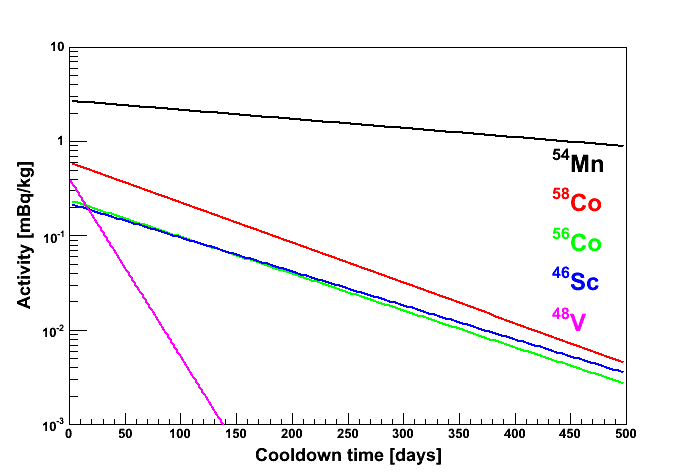
\includegraphics[width=0.475\linewidth]{plots/CosmogenicsSteel/CosmogenicsSteel_SeaLevel.png}
%\label{figCosmogenicsSteelDecays_1}}
%\subfigure[LNGS altitudel]{
%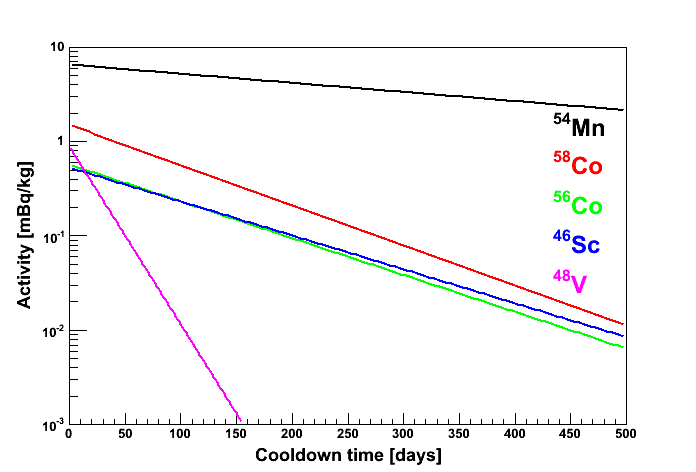
\includegraphics[width=0.475\linewidth]{plots/CosmogenicsSteel/CosmogenicsSteel_LNGSlevel.png}
%\label{figCosmogenicsSteelDecays_2}}
%\caption[Decays of the cosmogenic isotopes in the stainless steel after activation at sea level and at LNGS altitude]{Decays of the cosmogenic isotopes in the stainless steel after activation at sea level (a) and at LNGS altitude (b).}
%\label{figCosmogenicsSteelDecays}
%\end{figure}

The decays of the radioactive isotopes produced in 316Ti SS by cosmogenic activation at sea level and at LNGS altitude are shown as a function of cooldown time in Fig.~\ref{figCosmogenicsSteelDecays_1}. The saturation activities from the measurements published in Ref.~\cite{SteelCosmogenics} have been assumed as the starting values. As it can be seen, if the detector components have not been stored underground for at least 100~days, the sensitivity of the experiment can be potentially limited by cosmogenic activities. 
In Fall 2009, the detector had been underground for $\sim$500~days. The decays of the cosmogenic isotopes have been simulated with GEANT4, assuming a uniform distribution within all detector components made from 316Ti SS. The energy spectra are shown in Fig.~\ref{figCosmogenicsSteelDecays_2}, assuming activation at LNGS altitude and 500~days of cooldown time underground. Due to relatively long half-life, only the $^{54}$Mn isotope imposes a potential danger for the experiment's  background, with a residual activity of 0.89~mBq/kg after sea level exposure, and 2.14~mBq/kg after activation at LNGS altitude. These results have been used as starting values for the explanation of the measured background spectrum (see Section~\ref{secDataMCcomparison}).

%\begin{floatingfigure}[l]{0.475\textwidth}
\begin{figure}[!h]
\centering
\subfigure[]{
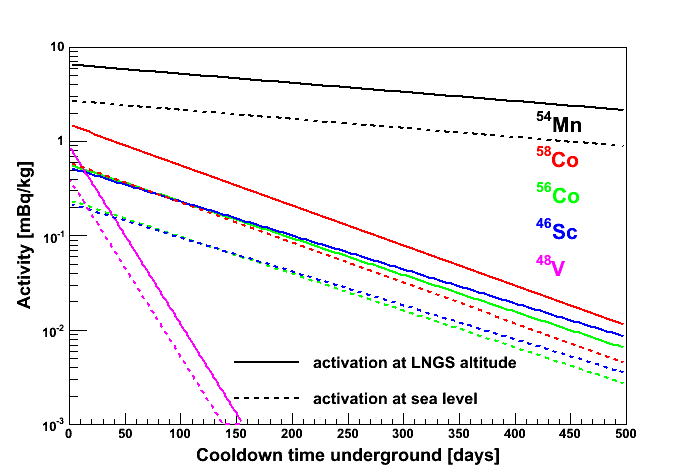
\includegraphics[width=0.475\linewidth]{plots/Cosmogenics/CosmogenicsSteel_LNGSandSEA.png}
\label{figCosmogenicsSteelDecays_1}}
\subfigure[]{
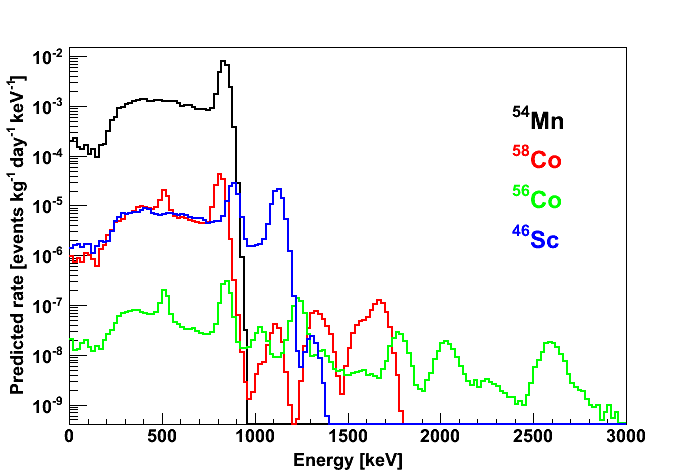
\includegraphics[width=0.475\linewidth]{plots/Cosmogenics/CosmogenicSpectra_LNGSproduction_noV48.png}
\label{figCosmogenicsSteelDecays_2}}
\caption[Decays of cosmogenic isotopes in the 316Ti stainless steel after activation at sea level and at LNGS altitude, and the energy spectra after cooldown of 500~days]{(a) - decays of cosmogenic isotopes in the 316Ti stainless steel after activation at sea level (solid lines) and at LNGS altitude (dashed lines). The measured production rates from Ref.~\cite{SteelCosmogenics} have been assumed as the start activities. (b) - energy spectra simulated with GEANT4 and assuming a cooldown time underground of 500~days. The spectra have been convoluted with the resolution of the combined energy scale of XENON100.}
\label{figCosmogenicsSteelDecays}
\end{figure}
%\end{floatingfigure}


%\begin{table}[!h]
%\centering
%\caption{Cosmogenic production in the 316Ti stainless steel from the measurements~\cite{SteelCosmogenics} and Monte Carlo simulations.}
%\label{tabSteelCosmogenics2}
%\vspace{0.2cm}
%\begin{tabular}{l | c | c }
%\hline
%Isotope				& \multicolumn{2}{c}{Activity after 500 days cooldown [mBq/kg]} \\
%					& sea level 				& LNGS level		\\
%\hline
%$^{54}$Mn			& 0.89					& 2.14 					\\
%$^{58}$Co 			& 4.5$\times$10$^{-3}$		& 1.13$\times$10$^{-2}$ 		\\
%$^{56}$Co 			& 2.7$\times$10$^{-3}$		& 6.4$\times$10$^{-3}$ 		\\
%$^{46}$Sc 			& 3.5$\times$10$^{-3}$		& 8.5$\times$10$^{-3}$ 		\\
%$^{48}$V 				& 1.5$\times$10$^{-10}$ 		& 3.3$\times$10$^{-10}$ 	\\
%\hline
%\end{tabular}
%\end{table}
